\frame{

\frametitle{\secname}
\begin{itemize}
\item Fourier Transform?
\begin{itemize}
\item Typically computed with complex numbers
\item Transform signal between time and frequency domain
\end{itemize}

\pause

\item This is not a math panel!
\begin{itemize}
\item See this 3Blue1Brown video:\\
``But what is the Fourier Transform? A visual introduction." $\rightarrow$
\smash[t]{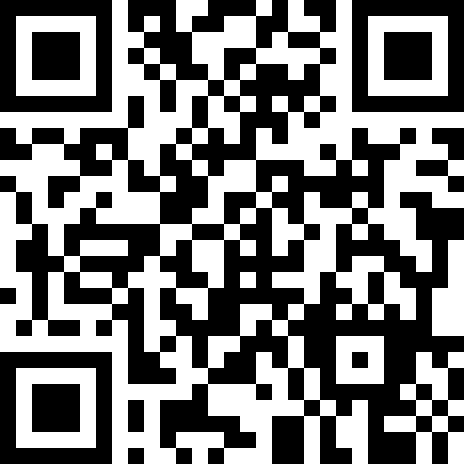
\includegraphics[width=0.2\linewidth]{slides/fft/qr_fourier_3b1b.png}}
\end{itemize}

\pause

\item This is an algorithms panel :3
\begin{itemize}
\item We will use \fft{} to multiply polynomials in $O(n\log n)$ time
\end{itemize}
\end{itemize}

}
